\documentclass[10pt,a4paper]{article}
\usepackage[utf8]{inputenc}
\usepackage[english,russian]{babel}
\usepackage{cmap}
\usepackage[OT1]{fontenc}
\usepackage{amsmath}
\usepackage{amsfonts}
\usepackage{amssymb}
\usepackage{graphicx}
\usepackage{float}
\usepackage{wrapfig}
\usepackage{caption}
\DeclareCaptionLabelSeparator{dot}{. }
\captionsetup{justification=centering,labelsep=dot}
\graphicspath{{pictures/}}
\DeclareGraphicsExtensions{.pdf,.png,.jpg,.eps}
\begin{document}

\part{Основы}



\textbf{4 Непараметрические фильтры}\\

Популярной альтернативой гауссовским методам являются \textit{непараметрические фильтры}. Непараметрические фильтры ограничены фиксированной функциональной формой апостериорного распределения, скажем, в виде гауссиана. Вместо этого, в них производится аппроксимация апостериорной вероятности конечным числом значений, каждое из которых примерно соответствует области в пространстве состояний. Некоторые непараметрические байесовские фильтры основаны на декомпозиции пространства состояний, когда каждое значение соответствует суммарной вероятности апостериорной плотности в компактной области пространства состояний. Другие алгоритмы аппроксимируют пространство состояний случайной выборкой из апостериорного распределения. Во всех случаях количество параметров, используемых для аппроксимации, может различаться. Качество аппроксимации напрямую зависит от количества параметров представления апостериорной вероятности. По мере увеличения количества параметров до бесконечности, при определённых условиях сглаживания, непараметрические методы равномерно сходятся к истинному значению апостериорной вероятности.

В этой главе обсуждаются два непараметрических подхода для аппроксимации апостериорных распределений в непрерывных пространствах с конечным количеством значений. В первом пространство состояний разбивается на конечное число областей и отображается на апостериорном распределении в виде гистограммы. На гистограмме каждому участку присваивается только одно значение суммарной вероятности, поэтому лучше всего представлять метод гистограмм как кусочно-постоянное приближение непрерывной плотности. Второй метод представляет апостериорные распределения в виде конечного множества элементов выборки. Результирующий фильтр известен под названием \textit{«многочастичного фильтра»} и приобрёл большую популярность в робототехнике. 

В обоих методах, гистограмм и многочастичных фильтров, не делается строгих параметрических заключений относительно апостериорной плотности, поэтому они хорошо приспособлены для представления сложных мультимодальных гипотез. Непараметрические методы часто являются наилучшим выбором, если робот сталкивается с проявлениями полной неопределённости и в случае возникновения серьёзных проблем ассоциации данных, порождающих отдельные, выраженные гипотезы. Однако, мощность представления эти методов достигается за счёт дополнительной вычислительной сложности. 

К счастью, в обоих непараметрических методах, описанных в этой главе, возможна настройка количества параметров согласно ожидаемой сложности апостериорного распределения. Когда апостериорное распределение имеет низкую сложность (например, сосредоточено вокруг одного значения с малым отклонением), используется лишь небольшое число параметров. Для комплексных апостериорных распределений с несколькими модами, разбросанными по пространству состояний, количество параметров сильно возрастёт. 

РЕСУРС-АДАПТИВНЫЕ АЛГОРИТМЫ

Методы, способные адаптировать количество параметров для отображения апостериорного распределения в реальном времени называются \textit{адаптивными}. Они называются \textit{ресурс-адаптивными}, если позволяют настраивать алгоритм соответственно доступным вычислительными ресурсам. 
Ресурс-адаптивные методы играют важную роль в робототехнике. Они открывают возможность для роботов принимать решения в реальном времени независимо от доступных вычислительных ресурсов. Многочастичные фильтры часто реализуются в виде ресурс-адаптивного алгоритмов, в которых количество частиц настраивается в процессе работы, основываясь на доступных вычислительных ресурсах.\\

\textbf{4.1 Histogram Filter}\\

Алгоритм \textit{Histogram filter} разбивает пространство состояний на конечное число областей и отображает суммарное апостериорное распределение для каждой области  в виде единственного значения вероятности. Для конечных пространств такие фильтры известны как \textit{дискретные байесовские фильтры}, а для непрерывных пространств обычно называют \textit{histogram filters}. Сначала опишем дискретные байесовские фильтры, а затем обсудим их использование в непрерывных пространствах состояний. \\

\textbf{4.1.1 Алгоритм дискретного байесовского фильтра}\\

\textit{Дискретные байесовские фильтры} применяются для задач с \textit{конечными} пространствами состояний, в которых случайная переменная $X_t$ может принимать конечное множество значений. Мы уже сталкивались с дискретным фильтром Байеса в Главе 2.4.2, обсуждая пример робота, оценивающего вероятность того, что дверь открыта. Некоторые из задач построения карт, обсуждаемые в более поздних главах, также включают дискретные случайные переменные. Например, в алгоритмах картографирования на основе карт занятости подразумевается, что каждая точка среды может быть либо занятой или свободной. Соответствующая случайная переменная имеет бинарный характер и может принимать одно из двух различных значений. Как видите, конечные пространства состояний играют важную роль в робототехнике.  

В Таблице 4.1 показан псевдокод дискретного байесовского фильтра. Этот код выводится из общего алгоритма байесовского фильтра в Таблице 2.1 путём замены интегрирования конечной суммой. Переменные $x_i$ и $x_k$ определяют отдельные состояния, которых может быть только конечное множество. 

\begin{table}[H]
\begin{center}
\begin{tabular}{|l|}
\hline
{}\\
1: \hspace{3mm} Algorithm Discrete\_ Bayes\_filter $(\{p_{k,t-1}\},u_t,z_t):$ \\
2: \hspace{7mm}\textit{for all $k$ do} \\
3: \hspace{12mm} $\bar{p}_{k,t}=\sum_i p(X_t=x_k|u_t,X_{t-1}=x_i)p_{i,t-1}$\\
4: \hspace{12mm} $p_{k,t}=\eta p(z_t|X_t=x_k)\bar{p}_{k,t}$\\
5: \hspace{7mm}\textit{endfor} \\
6:\hspace{7mm}
\textit{return} $\{p_{k,t}\}$\\
{}\\
\hline
\end{tabular}
\caption{(Таблица 4.1 Дискретный байесовский фильтр. Здесь $x_i$, $x_k$ определяют отдельные состояния. )}
\end{center}
\end{table}

Гипотеза в момент времени $t$ – это представление вероятности для каждого состояния $x_k$, и обозначается $p_{k,t}$. Поэтому, на вход алгоритма поступает дискретное распределение вероятности ${p_{k,t}}$, наряду с последними данными управляющего воздействия $u_t$ и измерения $z_t$. В строке 3 вычисляется прогноз, гипотеза относительно нового состояния, пока на основе одного лишь управляющего воздействия. Этот прогноз затем обновляется в строке 4 с учётом измерения.

СКРЫТАЯ МАРКОВСКАЯ МОДЕЛЬ

Алгоритм дискретного байесовского фильтра популярен во многих областях обработки сигналов, где часто именуется проходом вперёд в\textit{ скрытой марковской модели}, или \textit{СММ}.\\

\textbf{4.1.2 Непрерывное состояние}\\

Особенный интерес представляет использование дискретных фильтров Байеса в качестве инструмента логической оценки для \textit{непрерывных} пространств состояний. Как было сказано ранее, такие фильтры называются \textit{histogram filters}. На Рис. 4.1 показано, как с помощью histogram filter отображается случайная переменная и её нелинейное преобразование. Показанная кривая - это приближение гауссиана с помощью нелинейной функции в виде гистограммы. Начальное гауссовское распределение разбито на 10 интервалов. То же самое было сделано для предполагаемого распределения, но в двух интервалах вероятность так близка к нулю, что не видна на схеме. На Рис. 4.1 для сравнения также показаны истинные непрерывные распределения.

Histogram filter разбивает непрерывное пространство состояний на конечное множество \textit{интервалов}, или \textit{областей}:\\

(4.1)
$$dom(X_t)=\text{х}_{1,t}\cup \text{х}_{2,t}\cup...\text{х}_{K,t}$$

Здесь $X_t$ означает уже знакомую случайную переменную, описывающую состояние робота в момент времени $t$. Функция $dom(X_t)$ определяет пространство состояний, которое является множеством возможных значений, которые может принимать $X_t$. Каждое значение $\text{x}_{k,t}$ описывает выпуклую область.
Вместе эти области образуют разбиение пространства состояний. Для каждого $i\neq k$
получаем $\text{x}_{i,t}\cap \text{x}_{k,t} =0$ и $\bigcup_k\text{x}_{k,t} = dom(X_t)$.

\begin{figure}[H]
	\center{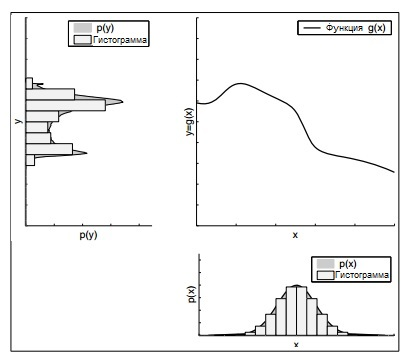
\includegraphics[width=1\linewidth]{41orig}}
	\caption{ (  Рис. 4.1 Отображение непрерывной случайной переменной в виде гистограммы. Закрашенная серым зона на нижней правой схеме изображает плотность непрерывной случайной переменной, $X$. Распределение плотности в виде гистограммы изображено с заполнением светло-серым цветом. Случайная переменная пропускается через функцию, изображённую на верхней правой схеме. Плотность и аппроксимация на гистограмме результирующей случайной переменной, $Y$, изображены на верхней левой схеме. Гистограмма преобразованной случайной переменной была вычислена путём передачи нескольких значений точек каждого интервала $X$ нелинейной функции.)}
	\label{fig:41orig}
\end{figure}

Очевидным разложением непрерывного пространства состояний является многомерная сетка, где каждое значение $\text{x}_{k,t}$ определяет ячейку сетки. Управляя разбиением такого представления, возможно настраивать баланс между точностью и вычислительной эффективностью. Разбиения с большим количеством ячеек имеют меньшую ошибку аппроксимации по сравнению с более грубыми, но, исключительно, за счёт возросшей вычислительной сложности.

Как уже обсуждалось, дискретный байесовский фильтр назначает каждой области 
$\text{x}_{k,t}$ единственную вероятность $p_{k,t}$, не сохраняя дополнительной информации о распределении оценки. Таким образом, апостериорное распределение становится кусочно-постоянной ФРВ, где вероятность каждого состояния $x_t$ в каждой области $\text{x}_{k,t}$ постоянна:\\

(4.2)
$$p(x_t)=\frac{p_{k,t}}{|\text{x}_{k,t}|}$$
	
Здесь $|\text{x}_{k,t}|$ означает площадь области $\text{x}_{k,t}$.

Если пространство состояний дискретно, условные вероятности $p(z_t|\text{x}_{k,t})$, $p(\text{x}_{k,t}|u_t, \text{x}_{i,t-1})$  чётко определены, и алгоритм может быть реализован в представленном виде. В непрерывных пространствах состояний обычно заданы плотности $p(x_t | u_t, x_{t-1})$ и $p(z_t | x_t)$, определённые для отдельных состояний (а не для областей пространства состояний). В тех случаях, когда все области $\text{x}_{k,t}$
малы и имеют одинаковый размер, эти плотности обычно аппроксимируются подставкой $\text{x}_{k,t}$ заменяющей функции. Например, можно просто «измерить» их с помощью среднего значения состояния в $\text{x}_{k,t}$\\

(4.3)
$$\hat{x}_{k,t}=|\text{x}_{k,t}|^{-1}\int_{\text{x}_{k,t}}x_t dx_t$$

А затем произвести следующую замену\\

(4.4)
$$p(z_t|\text{x}_{k,t})\approx p(z_t|\hat{x}_{k,t})$$

(4.5)
$$p(\text{x}_{k,t}|u_t,\text{x}_{i,t-1})\approx\eta\,|\text{x}_{k,t}|\,p(\hat{x}_{k,t}|u_t,\hat{x}_{i,t-1})$$

Эти аппроксимации являются результатом кусочно-однородной интерпретации дискретного байесовского фильтра в (4.2), и аналога приближения разложением в ряд Тейлора, который используется в EKF.\\

\textbf{4.1.3 Математический вывод приближения с помощью гистограммы }\\

Чтобы доказать применимость приближения (4.4), нужно обратить внимание, что $p(z_t | \text{x}_{k,t})$ можно выразить следующим интегралом:\\

(4.6)
\begin{equation*}
\begin{split}
p(z_t|\text{x}_{k,t})&=\frac{p(z_t,\text{x}_{k,t})}{p(\text{x}_{k,t})}\\
&=\frac{\int_{\text{x}_{k,t}} p(z_t,x_t)dx_t}{\int_{\text{x}_{k,t}}p(x_t)dx_t}\\
&=\frac{\int_{\text{x}_{k,t}} p(z_t|x_t)p(x_t)dx_t}{\int_{\text{x}_{k,t}}p(x_t)dx_t}\\
&\stackrel{(4.2)}{=}\frac{\int_{\text{x}_{k,t}} p(z_t|x_t)\frac{p_{k,t}}{|\text{x}_{k,t}|}dx_t}{\int_{\text{x}_{k,t}}\frac{p_{k,t}}{|\text{x}_{k,t}|}dx_t}\\
&=\frac{\frac{p_{k,t}}{|\text{x}_{k,t}|}}{\frac{p_{k,t}}{|\text{x}_{k,t}|}}\,\frac{\int_{\text{x}_{k,t}} p(z_t|x_t)dx_t}{\int_{\text{x}_{k,t}}1dx_t}\\
&=|\text{x}_{k,t}|^{-1}\int_{\text{x}_{k,t}}p(z_t|x_t)dx_t
\end{split}
\end{equation*}

Это выражение является точным описанием искомой вероятности для модели кусочно-однородного распределения в (4.2). Если сейчас аппроксимировать $p(z_t |
x_t)$ через $p(z_t | \hat{x}_{k,t})$ для $x_t\in \text{x}_{k,t}$, получим\\

(4.7)
\begin{equation*}
\begin{split}
p(z_t|\text{x}_{k,t})&\approx|\text{x}_{k,t}|^{-1}\int_{\text{x}_{k,t}}p(z_t|\hat{x}_{k,t})dx_t\\
&=|\text{x}_{k,t}|^{-1}p(z_t|\hat{x}_{k,t})\int_{\text{x}_{k,t}}1dx_t\\
&=|\text{x}_{k,t}|^{-1}p(z_t|\hat{x}_{k,t})|\text{x}_{k,t}|\\
&=p(z_t|\hat{x}_{k,t})
\end{split}
\end{equation*}
что и даёт, в результате, выражение, указанное выше в (4.4).

Вывод аппроксимации для $p(\text{x}_{k,t} | u_t, \text{x}_{i,t-1})$ в (4.5) несколько сложнее, поскольку области находятся по обеим сторонам искомой кривой. По аналогии с преобразованием выше, получим:\\

(4.8)
\begin{equation*}
\begin{split}
p(\text{x}_{k,t}&|u_t,\text{x}_{i,t-1})=\frac{p(\text{x}_{k,t},\text{x}_{i,t-1}|u_t)}{p(\text{x}_{i,t-1}|u_t)}\\
&=\frac{\int_{\text{x}_{k,t}}\int_{\text{x}_{i,t-1}}p(x_t,x_{t-1}|u_t)dx_t,dx_{t-1}}{\int_{\text{x}_{i,t-1}}p(x_{t-1}|u_t)dx_{t-1}}\\
&=\frac{\int_{\text{x}_{k,t}}\int_{\text{x}_{i,t-1}}p(x_t|u_t,x_{t-1})p(x_{t-1}|u_t)dx_t,dx_{t-1}}{\int_{\text{x}_{i,t-1}}p(x_{t-1}|u_t)dx_{t-1}}
\end{split}
\end{equation*}

Используем марковское свойство, постулирующее независимость между $x_{t-1}$ и $u_t$, получив $p(x_{t-1}|u_t)=p(x_{t-1})$:\\

(4.9)
\begin{equation*}
\begin{split}
&p(\text{x}_{k,t}|u_t,\text{x}_{i,t-1})\\
&=\frac{\int_{\text{x}_{k,t}}\int_{\text{x}_{i,t-1}}p(x_t|u_t,x_{t-1})p(x_{t-1})dx_t,dx_{t-1}}{\int_{\text{x}_{i,t-1}}p(x_{t-1})dx_{t-1}}\\
&=\frac{\int_{\text{x}_{k,t}}\int_{\text{x}_{i,t-1}}p(x_t|u_t,x_{t-1})\frac{p_{i,t-1}}{|\text{x}_{i,t-1}|}dx_t,dx_{t-1}}{\int_{\text{x}_{i,t-1}}\frac{p_{i,t-1}}{|\text{x}_{i,t-1}|}dx_{t-1}}\\
&=\frac{\int_{\text{x}_{k,t}}\int_{\text{x}_{i,t-1}}p(x_t|u_t,x_{t-1})dx_t,dx_{t-1}}{\int_{\text{x}_{i,t-1}}1dx_{t-1}}\\
&=|\text{x}_{i,t-1}|^{-1}\int_{\text{x}_{k,t}}\int_{\text{x}_{i,t-1}}p(x_t|u_t,x_{t-1})dx_t,dx_{t-1}
\end{split}
\end{equation*}

Если теперь аппроксимировать $p(x_t | u_t, x_{t-1})$ с помощью $p(\hat{x}_{k,t}|u_t,\hat{x}_{i,t-1})$ как было сделано раньше, получим следующее приближение. Обратите внимание на необходимость нормализующего члена $\eta$, который гарантирует, что аппроксимация будет допустимым вероятностным распределением:\\

(4.10)
\begin{equation*}
\begin{split}
&p(\text{x}_{k,t}|u_t,\text{x}_{i,t-1})\\
&\approx\eta|\text{x}_{i,t-1}|^{-1}\int_{\text{x}_{k,t}}\int_{\text{x}_{i,t-1}} p(\hat{x}_{k,t}|u_t,\hat{x}_{i,t-1})dx_t,dx_{t-1}\\
&=\eta|\text{x}_{i,t-1}|^{-1}p(\hat{x}_{k,t}|u_t,\hat{x}_{i,t-1})\int_{\text{x}_{k,t}}\int_{\text{x}_{i,t-1}}1dx_t,dx_{t-1}\\
&=\eta|\text{x}_{i,t-1}|^{-1}p(\hat{x}_{k,t}|u_t,\hat{x}_{i,t-1})|\text{x}_{k,t}|\,|\text{x}_{i,t-1}|\\
&=\eta|\text{x}_{k,t}|\,p(\hat{x}_{k,t}|u_t,\hat{x}_{i,t-1})
\end{split}
\end{equation*}

Если все области имеют одинаковый размер, (то есть $|\text{x}_{k,t}|$ одинаково для всех $k$), множитель $|\text{x}_{k,t}|$ можно просто вычеркнуть, учтя с помощью нормализующего члена. Результирующий дискретный байесовский фильтр эквивалентен алгоритму в Таблице 4.1. В приведённой реализации вспомогательные параметры $\bar{p}_k$ не образуют вероятностного распределения, поскольку они не нормализированы (ср. строку 3 с (4.10)). Тем не менее, нормализация выполняется в строке 4, поэтому выходные параметры представляют собой верное вероятностное распределение.\\

\begin{figure}[H]
	\center{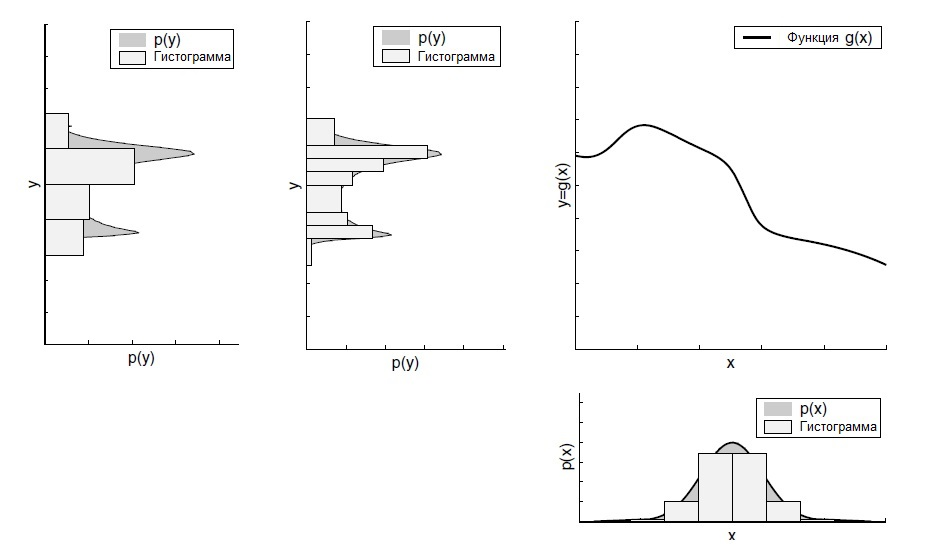
\includegraphics[width=1\linewidth]{42orig}}
	\caption{ (  Рис. 4.2 Динамическое и статическое разбиение. На верхней левой схеме показана гистограмма статической аппроксимации случайной переменной $Y$, построенная из 10 разбиений для покрытия площади $Y$ (6 разбиений имеют вероятность около нуля). На верхней схеме в середине показано представление некой случайной переменной в виде дерева, используя то же разбиение. )}
	\label{fig:42orig}
\end{figure}

\textbf{4.1.4 Методы разбиения}\\

В робототехнике используется два основных способа разбиения непрерывных пространств состояний: \textit{статические} и \textit{динамические}. Статические методы полагаются на фиксированное, предварительное выбранное разбиение, вне зависимости от формы апостериорного разбиения, которое необходимо аппроксимировать. Динамические методы используют адаптацию разбиения для конкретной формы апостериорного распределения. Статические методы обычно проще применять, но они могут весьма расточительно расходовать вычислительные ресурсы.\\
ДЕРЕВЬЯ ПЛОТНОСТИ

Показательным примером метода динамического разбиения является семейство \textit{деревьев плотности}. В деревьях плотности пространство состояний разбивается рекурсивно, отражая вероятностную меру апостериорного распределения. Идея такого разбиения состоит в том, чтобы уровень детализации разбиения отражал свойства апостериорного распределения: чем меньше вероятность региона, тем грубее разбиение. На Рис. 4.2 показана разница между представлением в виде статичной сетки и дерева плотностей. В силу более компактного представления дерево плотностей позволяет, при одинаковом разбиении, получить более высокое качество аппроксимации. Кроме того, динамические методы, такие как деревья плотностей, часто позволяют на порядок снизить вычислительную сложность по сравнению со статическими, хотя и требуют дополнительных усилий в реализации.\\
ВЫБОРОЧНОЕ ОБНОВЛЕНИЕ

Похожий эффект  может быть достигнут  
\textit{выборочным обновлением}. При обновлении апостериорного распределения, выраженного в виде сетки, затрагивается только часть всех ячеек сетки. В обычной реализации такого метода обновляются только те ячейки, апостериорная вероятность которых превосходит определяемый пользователем порог.

Выборочное обновление можно рассматривать как гибридное разбиение пространства состояний на мелкую сетку и единственное большое множество, содержащее все области не затрагиваемые процедурой выборочного обновления. В этом свете его можно воспринимать как метод динамического разбиения, поскольку решение о том, какие ячейки следует обновлять, принимается в реальном времени, на основе формы апостериорного распределения. Методы выборочного обновления позволяют на порядки уменьшить задействованные при обновлении оценок вычислительные мощности  и использовать разбиение в виде сеток для пространств с тремя или более измерениями.  
 
В литературе по мобильной робототехнике часто различаются \textit{топологические} и \textit{метрические}
представления пространства. Хотя точного формального определения этих терминов нет, топологические отображения часто представляют в виде графов, где узлы соответствуют некоторым значимым местам (или признакам) окружающей среды. В замкнутых пространствах это могут быть пересечения, разветвления, тупики и так далее. Таким образом, разрешение разбиений зависит от структуры окружающей среды. Альтернативным способом является разбиение пространства состояний сетками с регулярной ячейкой. Такое разбиение не зависит от формы и расположения ориентиров окружающей среды. Отображения в виде сеток часто именуют метрическими, хотя, строго говоря, метрическими являются состояния, а не разбиения. В мобильной робототехнике пространственное разрешение сеток обычно выше, чем у топологических представлений. Скажем, в некоторых примерах в Главе 7 используются сетки с размером ячейки 10 см или менее. Дополнительная точность при этом достигается ценой возросшей вычислительной сложности.\\ 

\begin{table}[H]
\begin{center}
\begin{tabular}{|l|}
\hline
{}\\
1: \hspace{3mm} Algorithm binary\_ Bayes\_filter $(l_{t-1},z_t):$ \\
2: \hspace{7mm}$l_t=l_{t-1}+\log\frac{p(x|z_t)}{1-p(x|z_t)}-\log\frac{p(x)}{1-p(x)}$\\
3:\hspace{7mm}$\textit{return} \,l_t$\\
{}\\
\hline
\end{tabular}
\caption{(Таблица 4.2 Бинарный фильтр Байеса в логарифмическом виде с инвертированной моделью измерений. Здесь $l_t$ - это логарифм шансов апостериорной оценки по бинарной переменной состояния, постоянной во времени. )}
	\end{center}
\end{table}

\textbf{4.2 Бинарные байесовские фильтры со статическим состоянием.}\\

Некоторые проблемы робототехники лучше всего формулировать в виде задач оценки с бинарным состоянием, постоянным во времени. Для решения этих задач предназначен \textit{бинарный фильтр Байеса}. Такие задачи возникают, если робот оценивает фиксированный бинарный параметр окружающей среды с помощью последовательности измерений датчика. Например, имеется необходимость узнать, открыта дверь или закрыта, в контексте, когда состояние двери в процессе измерения не меняется. 

КАРТЫ СЕТКИ ЗАНЯТОСТИ

Другим примером бинарных фильтров Байеса со статическим состоянием являются \textit{карты сеток занятости}, с которыми мы столкнёмся в Главе 9.

Когда состояние статично, оценка является лишь функцией измерений:\\
 
(4.11)
$$bel_t(x)=p(x|z_{1:t},u_{1:t})=p(x|z_{1:t})$$

где состояние выбирается из двух возможных значений, обозначаемых $x$ и $\neg x$. Очевидно, что $bel_t(\neg x) = 1 - bel_t(x)$. Отсутствие индекса времени для состояния $x$ отображает тот факт, что состояние не изменяется со временем.

ЛОГАРИФМ ОТНОШЕНИЯ ШАНСОВ

Обычно, задачи бинарной оценки такого вида  возможно разрешить, используя дискретный фильтр Байеса из Таблицы 4.1. Оценка, обычно, задаётся как 
\textit{логарифм отношения шансов}. Шансы состояния $x$ определяются в виде отношения вероятности данного события и вероятности его противоположности
$p(x)$\\

(4.12)
$$\frac{p(x)}{p(\neg x)} = \frac{p(x)}{1-p(x)}$$

Логарифм шансов - это логарифм следующего выражения\\

(4.13)
$$l(x):=\log\frac{p(x)}{1-p(x)}$$

Логарифм шансов принимает значения от$-\infty$ до $\infty$. Байесовский фильтр для обновления оценок в представлении логарифма шансов имеет вычислительно лаконичный вид, обходя проблему отсекания вероятностей, близких к 0 или 1.

В Таблице 4.2 приведён основной алгоритм обновления. Он аддитивен, и, практически, любой алгоритм, в котором происходит приращение или уменьшение переменной в качестве реакции на измерения, может быть интерпретирован как байесовский фильтр в форме логарифма шансов.\\ 
ИНВЕРТИРОВАННАЯ МОДЕЛЬ ИЗМЕРЕНИЙ\\
Этот бинарный байесовский фильтр использует \textit{инвертированную модель измерений} $p(x | z_t)$, вместо известной прямой модели $p(z_t | x)$. Инвертированная модель измерений определяет распределение  бинарной переменной состояния в виде функции измерения $z_t$.

Инверсные модели часто используются в ситуациях с более сложными, чем бинарное состояние, измерениями. Примером такой ситуации является проблема определения, закрыта дверь или нет, используя изображения с камеры. Само состояние очень простое, но пространство всех измерений огромно. Проще найти функцию, которая вычисляет вероятность того, что дверь закрыта, на основании изображения с камеры, чем описывать распределение по всем изображениям с камеры, на которых имеется закрытая дверь. Другими словами, легче применить инвертированную модель датчика, чем прямую. 

Как читатель может легко проверить, воспользовавшись определением логарифма шансов в (4.13), оценку $bel_t(x)$ можно восстановить из отношения логарифма шансов $l_t$ с помощью следующего равенства:\\

(4.14)
$$bel_t(x)=1-\frac{1}{1+\exp\{l_t\}}$$

Чтобы проверить корректность нашего алгоритма бинарного фильтра Байеса, кратко переформулируем основное уравнение фильтра, явно указав нормализующий член:\\

(4.15)
\begin{equation*}
\begin{split}
p(x|z_{1:t})&=\frac{p(z_t|x,z_{1:t-1})\,p(x|z_{1:t-1})}{p(z_t|z_{1:t-1})}\\
&=\frac{p(z_t|x)\,p(x|z_{1:t-1})}{p(z_t|z_{1:t-1})}
\end{split}
\end{equation*}

Применим теорему Байеса к модели измерений $p(z_t|x)$:\\

(4.16)
$$p(z_t|x)=\frac{p(x|z_t)\,p(z_t)}{p(x)}$$

и получим\\

(4.17)
$$p(x|z_{1:t})=\frac{p(x|z_t)\,p(z_t)\,p(x|z_{1:t-1})}{p(x)\,p(z_t|z_{1:t-1})}$$

По аналогии, есть противоположное событие $\neg x$:\\

(4.18)
$$p(\neg x|z_{1:t})=\frac{p(\neg x|z_t)\,p(z_t)\,p(\neg x|z_{1:t-1})}{p(\neg x)\,p(z_t|z_{1:t-1})}$$

Деление (4.17) на (4.18) позволяет сократить различные сложные для вычисления вероятности:\\

(4.19)
\begin{equation*}
\begin{split}
\frac{p(x|z_{1:t})}{p(\neg x|z_{1:t})}&=\frac{p(x|z_t)}{p(\neg x|z_t)}\,\frac{p(x|z_{1:t-1})}{p(\neg x|z_{1:t-1})}\,\frac{p(\neg x)}{p(x)}\\
&=\frac{p(x|z_t)}{1-p(x|z_t)}\,\frac{p(x|z_{1:t-1})}{1-p(x|z_{1:t-1})}\,\frac{1-p(x)}{p(x)}
\end{split}
\end{equation*}

Определим отношение логарифма шансов оценки $bel_t(x)$ через $l_t(x)$. Оценка в момент времени $t$ задаётся следующим логарифмом (4.19).\\

(4.20)
\begin{equation*}
\begin{split}
l_t(x)&=\log\frac{p(x|z_t)}{1-p(x|z_t)}+\log\frac{p(x|z_{1:t-1})}{1-p(x|z_{1:t-1})}+\log\frac{1-p(x)}{p(x)}\\
&=\log\frac{p(x|z_t)}{1-p(x|z_t)}-\log\frac{p(x)}{1-p(x)}+l_{t-1}(x)
\end{split}
\end{equation*}

Здесь $p(x)$ - априорная вероятность состояния $x$. Как и в (4.20), каждое обновление измерения включает добавление априорной вероятности (в форме логарифма шансов). Априорная вероятность также определяет логарифм шансов начальной оценки перед обработкой каких-либо измерений датчиков:\\

(4.21)
$$l_0(x)=\log\frac{p(x)}{1-p(x)}$$\\

\textbf{4.3 Многочастичный фильтр}\\

\textbf{4.3.1 Общий алгоритм}\\

\textit{Многочастичный фильтр} является альтернативой непараметрической реализации байесовского фильтра. Также как фильтр на основе гистограмм, многочастичный фильтр аппроксимирует апостериорную вероятность с помощью конечного числа параметров. Различие состоит в способе генерации и распределения в пространстве состояний. Ключевая идея многочастичного фильтра состоит в отображении апостериорной вероятности $bel(x_t)$ с помощью выборки случайных значений состояния этого апостериорного распределения. На Рис. 4.3 принцип показан на примере гауссовой функции. Вместо представления распределения в параметрической форме, например, экспоненциальной функции, определяющей плотность нормального распределения, многочастичные фильтры представляют распределения с помощью выборки из них. Такое распределение является приближенным, но оно непараметрическое, а, значит, способно отображать значительно более широкое пространство распределений, чем, к примеру, гауссовы функции. Другим преимуществом отображения на основе выборки является возможность моделирования нелинейных преобразований случайных переменных, что показано на Рис. 4.3.\\
\begin{figure}[H]
	\center{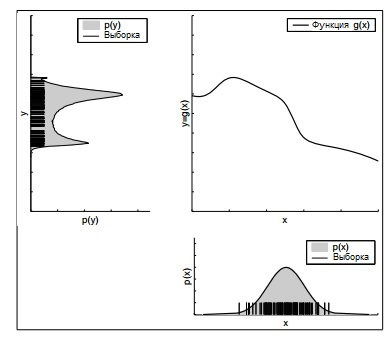
\includegraphics[width=1\linewidth]{43orig}}
	\caption{ (  Рис. 4.3 Отображение в виде «частицы», используемое в многочастичных фильтрах. На нижней правой схеме показаны элементы выборки, извлечённые из гауссовской случайной переменной, $X$. Эти элементы пропускаются через нелинейную функцию, показанную сверху справа. Результирующие элементы распределены согласно случайной переменной $Y$.)}
	\label{fig:43orig}
\end{figure}
 
В многочастичных фильтрах выборка из апостериорного распределения называется частицами
и обозначается как\\

(4.22)
$$\mathcal X_t:=x_t^{[1]},x_t^{[2]},...,x_t^{[M]}$$

Каждая частица $x_t^{[m]}$ (с $1\leq m\leq M)$ является конкретным экземпляром состояния в момент времени $t$. Другими словами, частица – это гипотеза относительно настоящего значения переменной среды в момент времени $t$. Здесь $M$ означает число частиц в множестве частиц $\mathcal X_t$. На практике, количество частиц $M$ часто достаточно велико, например, $M = 1000$. В некоторых реализациях $M$ является функцией времени или других количественных характеристик, относящихся к оценке $bel(x_t)$.\\

\begin{table}[H]
\begin{center}
\begin{tabular}{|l|}
\hline
{}\\
1: \hspace{3mm} Algorithm Particle\_filter $(\mathcal X_{t-1},u_t,z_t):$ \\
2:\hspace{7mm}$\bar{\mathcal X}_t=\mathcal X_t=0$\\
3:\hspace{7mm}$\textit{for }\, m=1\, \textit{to}\, M\,\textit{do}$\\
4:\hspace{12mm}$\textit{sample }\,x_t^{[m]}\sim p(x_t|u_t,x_{t-1}^{[m]})$\\
5:\hspace{12mm}$w_t^{[m]}=p(z_t|x_t^{[m]})$\\
6:\hspace{12mm}$\bar{\mathcal X}_t=\bar{\mathcal X}_t+\langle x_t^{[m]},w_t^{[m]}\rangle$\\
7:\hspace{7mm}\textit{endfor}\\
8:\hspace{7mm}$\textit{for }\, m=1\, \textit{to}\, M\,\textit{do}$\\
9:\hspace{12mm}$\textit{draw } \,i\, \textit{with probability} \propto w_t^{[i]}$\\
10:\hspace{12mm}$\textit{add }\, x_t^{[i]}\, \textit{to}\, \mathcal X_t$\\
11:\hspace{7mm}\textit{endfor}\\
3:\hspace{7mm}$\textit{return}\, \mathcal X_t$\\
{}\\
\hline
\end{tabular}
\caption{(Таблица 4.3 Алгоритм многочастичного фильтра, вариант байесовского фильтра, основанного на выборке по значимости. )}
\end{center}
\end{table}
Основная идея фильтров частиц лежит в аппроксимации оценки $bel(x_t)$ с помощью набора частиц $\mathcal X_t$. В идеальном случае, правдоподобие гипотезы состояния $x_t$ на основе набора частиц $\mathcal X_t$, будет пропорционально апостериорному распределению байесовского фильтра 
$bel(x_t)$:\\

(4.23)
$$x_t^{[m]}\,\sim\,p(x_t|z_{1:t},u_{1:t})$$

Как следствие (4.23), чем плотнее область пространства состояний заполнена выборкой, тем более вероятно, что настоящее состояние попадёт в эту область. 
Как будет обсуждаться ниже, свойство (4.23) для стандартного алгоритма многочастичного фильтра сохраняется лишь асимптотически при
$M\uparrow\infty$. Для конечного $M$ частицы выбираются из несколько другого распределения, но на практике разница несущественна, пока количество частиц не станет слишком малым (то есть, $M\geq100$).

Так же, как во всех других алгоритмах байесовских фильтров, обсуждаемых ранее, алгоритм многочастичного фильтра рекурсивно строит оценку $bel(x_t)$ из оценки $bel(x_{t-1})$,
взятой на шаг ранее. Поскольку оценки отображены наборами частиц, это означает, что многочастичные фильтры рекурсивно строят набор частиц $\mathcal X_t$ из набора $\mathcal X_{t-1}$.

Самый общий вариант многочастичного фильтра приведён в Таблице 4.3.
На вход этого алгоритма подаётся набор частиц $\mathcal X_{t-1}$, вместе с последними данными управляющего воздействия $u_t$ и последними данными измерений $z_t$. Затем алгоритм строит временный набор частиц $\bar{\mathcal X}$, отображающий оценку $\overline{bel}(x_t)$. Это выполняется путём систематической обработки каждой частицы $x_{t-1}^{[m]}$ во входном наборе частиц $\mathcal X_{t-1}$. Далее эти частицы трансформируются в набор $\mathcal X_t$, который аппроксимирует апостериорное распределение $bel(x_t)$. Это происходит следующим образом:\\

1. В строке 4 генерируется гипотетическое состояние $x_t^{[m]}$ для момента времени $t$, используя частицу 
$x_{t-1}^{[m]}$ и управляющее воздействие $u_t$. Результирующий образец индексируется по $m$, чтобы показать, что он был сгенерирован из $m$-ой частицы в $\mathcal X_{t-1}$. На этом шаге выполняется выборка из распределения переходов состояний $p(x_t | u_t, x_{t-1})$. Для выполнения этого шага необходимо взять выборку из распределения. Набор частиц, полученный после $M$ итераций представляет собой отображение оценки фильтра $\overline{bel}(x_t)$.\\

ФАКТОР ЗНАЧИМОСТИ \\
2. В строке 5 для каждой частицы $x_t^{[m]}$ вычисляется так называемый \textit{фактор значимости}, обозначаемый $w_t^{[m]}$. Факторы значимости используются для учёта измерения 
$z_t$ в наборе частиц. Таким образом, значимость – это вероятность измерения $z_t$ в частице $x_t^{[m]}$, заданной $w_t^{[m]} = p(z_t | x_t^{[m]})$. Если интерпретировать $w_t^{[m]}$ как вес частицы, набор взвешенных частиц представляет (приближённо) апостериорную вероятность байесовского фильтра $bel(x_t)$.\\

ПЕРЕВЫБОРКА\\
3. Настоящий «фокус» многочастичного фильтра происходит в строках с 8 по 11 в Таблице 4.3 в процессе, известном как перевыборка
или выборка по значимости. Алгоритм извлекает с заменой $M$ частиц из временного набора $\bar{\mathcal X}_t$, причём вероятность извлечения частицы из набора задана ее весом значимости. При перевыборке происходит преобразование набора $M$ в другой набор частиц такого же размера. Распределение частиц изменяется с учётом весов значимости: там, где до перевыборки частицы были распределены согласно $\overline{bel}(x_t)$, после неё распределение будет примерно соответствовать апостериорному
$bel(x_t) =\eta\, p(z_t | x_t^{[m]})\overline{bel}(x_t)$.
В результирующей выборке появляется много дубликатов, поскольку частицы извлекаются с заменой. Более важно, что имеются и частицы не включённые в $\mathcal X_t$: это частицы с весом значимости ниже порогового.

Этап перевыборки выполняет важную функцию возврата частиц обратно в апостериорное распределение $bel(x_t)$. Фактически, альтернативная (и обычно худшая) версия многочастичного фильтра может никогда не выполнять перевыборку, а, вместо этого, поддерживать для каждой частицы многократно обновляемый вес значимости, инициализированный единицей:\\

(4.24)
$$w_t^{[m]}=p(z_t|x_t^{[m]})\,w_{t-1}^{[m]}$$

Такой алгоритм многочастичного фильтра будет в состоянии аппроксимировать апострериорное распределение, но многие частицы окажутся в областях с малой апостериорной вероятностью. 
В результате, потребуется значительно больше частиц, а их точное количество зависит от апостериорного распределения. Шаг перевыборки – это вероятностная реализация дарвинской идеи \textit{выживания сильнейшего}: он перенаправляет набор частиц в области пространства состояний с высокой апостериорной вероятностью. Таким образом, вычислительные ресурсы алгоритма фильтрации сосредоточены на тех областях пространства состояний, где они нужнее всего.\\

\textbf{4.3.2 Перевыборка на основе значимости }\\

Для вывода многочастичного фильтра, будет полезным обсудить этап перевыборки более детально.

На первый взгляд, мы сталкиваемся с задачей вычисления ожидания по функции плотности вероятности $f$, по имеющейся другой функции плотности вероятности, $g$. Например, необходимо найти ожидание $x\in A$. Можно выразить эту вероятность в виде ожидания по $g$. Здесь $I$ – это индикаторная функция, которая принимает значение 1, если аргумент верен, и 0 - в остальных случаях.\\

(4.25)
\begin{equation*}
\begin{split}
E_f[I(x\in A)]&=\int f(x) I(x\in A)dx\\
&=\int\underbrace{\frac{f(x)}{g(x)}}_{=:w(x)}\,g(x)\,I(x\in A)dx\\
&=E_g[w(x)\,I(x\in A)]
\end{split}
\end{equation*}

Здесь $w(x)=\frac{f(x)}{g(x)}$ это весовой коэффициент, который отражает "нестыковку" между $f$ и $g$. Чтобы это равенство было верным, необходимо, чтобы $f(x)>0\longrightarrow
g(x)>0$.

ЦЕЛЕВОЕ РАСПРЕДЕЛЕНИЕ\\
Это преобразование выполняется алгоритмом перевыборки по значимости. На Рис. 4.4a показана функция плотности $f$ вероятностного распределения, которая
здесь и далее будет называться \textit{целевым распределением}. Как и прежде, мы хотели бы получить значение из $f$, но, напрямую сделать это невозможно. Вместо этого будем генерировать частицы из плотности $g$, как показано на
Рис. 4.4b.\\

\begin{figure}[H]
	\center{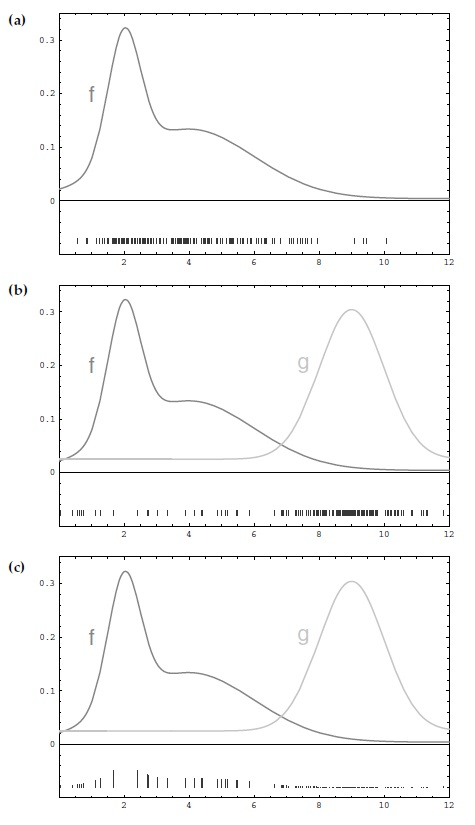
\includegraphics[width=0.83\linewidth]{44orig}}
	\caption{ (  Рис. 4.4 Иллюстрация факторов значимости в многочастичных фильтрах: (a) Необходимо аппроксимировать целевую плотность $f$. (b) Вместо получения значений из $f$ напрямую, мы можем только генерировать выборку из другой функции, $g$. Выборка из $g$ показана внизу схемы. (c) Выборка из $f$ получается назначением веса
	$f(x)/g(x)$ каждому значению $x$. В многочастичных фильтрах $f$ соответствует оценке $bel(x_t)$, а $g$ – оценке $\overline{bel}(x_t)$.)}
	\label{fig:44orig}
\end{figure}

ПРЕДЛАГАЕМОЕ РАСПРЕДЕЛЕНИЕ

Распределение, которое соответствует плотности $g$, называется \textit{предлагаемое распределение}. Плотность $g$ должна быть такой, чтобы $f(x) > 0$ и $g(x) > 0$, гарантируя ненулевую вероятность сгенерировать частицу при формировании выборки из $g$ для любого состояния, которое может быть сгенерировано при выборке из $f$. Таким образом,
результирующий набор частиц, показанный внизу на Рис. 4.4b, распределён согласно $g$, а не $f$. В частности, для любого интервала $A\subseteq dom(X)$ (или, в более общем виде, любого борелевского множества $A$) эмпирическое количество частиц, попадающих в $A$, сходится к интегралу $g$ под $A$:\\

(4.26)
$$\frac{1}{M}\sum_{m=1}^M I(x^{[m]}\in A)\longrightarrow\int_A g(x)dx$$

Чтобы распределить эту разность между $f$ и $g$, частицы $x^{[m]}$  взвешиваются следующим коэффициентом\\

(4.27)
$$w^{[m]}=\frac{f(x^{[m]})}{g(x^{[m]})}$$

Это показано на Рис 4.4c: вертикальные полоски на схеме обозначают величину весов значимости. Веса значимости – это ненормализованная масса вероятности каждой частицы. В частности, получается выражение\\

(4.28)
$$\left[ \sum_{m=1}^M w^{[m]}\right] ^{-1}\sum_{m=1}^M I(x^{[m]}\in A)w^{[m]}\longrightarrow\int_A f(x)dx$$

в котором первый член служит нормализующим для всех весов значимости. Другими словами, несмотря на то, что мы генерируем частицы из плотности $g$, приблизительно взвешенные частицы сходятся к плотности $f$. Можно показать, что в общих условиях, эта аппроксимация сходится к искомой $E_f[I(x\in A)]$ для произвольных наборов $A$. В большинстве случаев, скорость сходимости находится в диапазоне $O(1/\sqrt{M})$, где $M$ – количество элементов. Постоянный множитель зависит от сходства $f(x)$ и $g(x)$.

В многочастичных фильтрах плотность $f$ связана с целевой оценкой $bel(x_t)$.
При асимптотически верном допущении, что частицы в $\mathcal X_{t-1}$ распределены согласно $bel(x_{t-1})$, плотность $g$ связана с распределением произведения:\\

(4.29)
$$p(x_t|u_t,x_{t-1}) bel(x_{t-1})$$

Это распределение оказывается предлагаемым распределением.\\

\textbf{4.3.3 Математический вывод многочастичного фильтра}\\

Для того, чтобы математически вывести многочастичные фильтры, полезно воспринимать частицы в виде элементов последовательностей состояний 

(4.30)
$$x_{0:t}^{[m]}=x_0^{[m]},x_1^{[m]},...,x_t^{[m]}$$

Легко модифицировать алгоритм соответствующим образом: просто добавим частицу
$x_t^{[m]}$ к последовательности элементов состояния, из которой было сгенерировано $x_{0:t-1}^{[m]}$. Этот многочастичный фильтр вычисляет апостериорное распределение по всем последовательностям состояния:\\

(4.31)
$$bel(x_{0:t})=p(x_{0:t}|u_{1:t},z_{1:t})$$

вместо оценки $bel(x_t) = p(x_t | u_{1:t}, z_{1:t})$. Очевидно, что пространство по всем последовательностям состояния имеет огромный размер, и пытаться полностью покрыть его частицами, как правило, не слишком продуктивная идея. 
Однако, здесь это нас не остановит, поскольку определение предназначено только для вывода алгоритма многочастичного фильтра в Таблице 4.3.

Апостериорная оценка $bel(x_{0:t})$ получается аналогично выводу $bel(x_t)$
в Главе 2.4.3. В частности,\\

(4.32)
\begin{equation*}
\begin{split}
&p(x_{0:t}|z_{1:t},u_{1:t})\\
&\stackrel{\text{Bayes}}{=}\eta\,p(z_t|x_{0:t},z_{1:t-1},u_{1:t})\,p(x_{0:t}|z_{1:t-1},u_{1:t})\\
&\stackrel{\text{Markov}}{=}\eta\,p(z_t|x_t)\,p(x_{0:t}|z_{1:t-1},u_{1:t})\\
&\hspace{3mm}=\eta\,p(z_t|x_t)\,p(x_t|x_{0:t-1},z_{1:t-1},u_{1:t})\,p(x_{0:t-1}|z_{1:t-1},u_{1:t})\\
&\stackrel{\text{Markov}}{=}\eta\,p(z_t|x_t)\,p(x_t|x_{t-1},u_t)\,p(x_{0:t-1}|z_{1:t-1},u_{1:t-1})
\end{split}
\end{equation*}

Обратите внимание на отсутствие знаков интеграла в выводе, что стало результатом сохранения в апостериорной оценке всех состояний, а не только последнего, как это было в Главе 2.4.3.

Теперь вывод можно выполнить, используя одну лишь индукцию. Начальное условие проверим, допустив, что первый набор частиц получается выборкой из апостериорной плотности $p(x_0)$. Пусть набор частиц в момент времени $t - 1$ распределён согласно $bel(x_{0:t-1})$. Для m-ой частицы $x_{0:t-1}^{[m]}$ в этом наборе, элемент $x_t^{[m]}$, сгенерированный на Шаге 4 нашего алгоритма, стал элементом предлагаемого распределения:\\

(4.33)
$$p(x_t|x_{t-1},u_t)bel(x_{0:t-1})=p(x_t|x_{t-1},u_t)\,p(x_{0:t-1}|z_{1:t-1},u_{1:t-1})$$

где\\

(4.34)
\begin{equation*}
\begin{split}
w_t^{[m]}&=\frac{\text{целевое распределение}}{\text{предлагаемое распределение}}\\
&=\frac{\eta\,p(z_t|x_t)\,p(x_t|x_{t-1},u_t)\,p(x_{0:t-1}|z_{1:t-1},u_{1:t-1})}{p(x_t|x_{t-1},u_t)\,p(x_{0:t-1}|z_{0:t-1},u_{0:t-1})}\\
&=\eta\,p(z_t|x_t)
\end{split}
\end{equation*}

Константа $\eta$ роли не играет, поскольку перевыборка выполняется для вероятностей, \textit{пропорциональных} весам значимости. В результате перевыборки частиц с вероятностями, пропорциональными $w_t^{[m]}$, результирующие частицы заведомо распределены согласно произведению предположительных весов и весов значимости $w_t^{[m]}$:\\

(4.35)
$$\eta\,w_t^{[m]}p(x_t|x_{t-1},u_t)\,p(x_{0:t-1}|z_{0:t-1},u_{0:t-1})=bel(x_{0:t})$$

(Обратите внимание, что постоянный множитель $\eta$ отличается от такого, приведённого в (4.34).) Алгоритм в Таблице 4.4 следует простому наблюдению, что, если $x_{0:t}^{[m]}$
распределено согласно $bel(x_{0:t})$, тогда элемент состояния $x_t^{[m]}$,  очевидно, распределён согласно $bel(x_t)$.

Как будет доказано ниже, этот вывод верен только при $M \uparrow \infty$, в силу произвольности в определении нормализующих постоянных. Тем не менее, даже при конечном числе $M$, он отражает идею многочастичного фильтра.\\

\textbf{4.3.4 Практические соображения и свойства многочастичных фильтров. Извлечение плотности}\\

Наборы элементов, поддерживаемые в многочастичных фильтрах, отображают дискретные аппроксимации непрерывных оценок. Однако, для многих реализаций требуется доступность непрерывных оценок, то есть не только состояний, представленных в наборе частиц, но произвольной точки пространства состояний. Задача извлечения непрерывной плотности из таких элементов называется оценкой плотности.
Проиллюстрируем в неформальном виде некоторые подходы к оценке плотности.

На Рис. 4.5 показаны различные способы извлечения плотности из частиц. 
На самой левой схеме показаны частицы и плотность преобразованной гауссовой функции из нашего стандартного примера с Рис. 4.3. Простой и очень эффективный метод извлечения плотности из таких частиц - это вычисление \textit{гауссова приближения}, как показано пунктиром на Рис. 4.5(b).
В этом случае, гауссова функция, полученная на основе частиц, практически идентична гауссову приближению настоящей плотности (сплошная линия).

АЛГОРИТМ К-СРЕДНИХ \\
Очевидно, гауссово приближение отражает лишь основные свойства плотности, и применимо только для одномодальной плотности. Мультимодальные распределения элементов требуют более сложных методов, таких как \textit{кластеризация по методу k-средних}, которая аппроксимирует плотность, используя смеси гауссианов. Альтернативный подход показан на Рис. 4.5(c). Здесь дискретная \textit{гистограмма} наложена на пространство состояний и вероятность каждого интервала вычисляется суммированием весов частиц, которые попадают в диапазон. По аналогии с фильтром на основе гистограмм, значительным недостатком такого подхода является факт экспоненциальной зависимости сложности пространства от числа измерений. С другой стороны, с помощью гистограмм возможно очень эффективно, в вычислительном смысле, отобразить многомерные распределения, а плотность любого состояния можно извлечь за время, не зависящее от числа частиц.

ДЕРЕВО ПЛОТНОСТЕЙ\\
Пространственная сложность представлений в виде гистограмм может быть существенно уменьшена с помощью генерации из частиц деревьев плотностей, как обсуждалось в Главе 4.1.4. Однако, деревья плотностей имеют логарифмическое к глубине дерева количество вычислительных операций в операциях поиска при извлечении плотности произвольной точки в пространстве состояний.

ОЦЕНКА ПЛОТНОСТИ ЯДРА\\ 
\textit{Оценка плотности ядра} - это ещё один способ преобразования набора частиц в непрерывную плотность. В этом методе каждая частица рассматривается в виде центра так называемого ядра, а общая плотность задана смесью плотностей ядер. На Рис. 4.5(d) показана смесь плотностей, получившаяся в результате размещения в каждой частице гауссового ядра. Преимуществом оценок плотности ядер является гладкость и алгоритмическая простота. При этом, сложность вычисления плотности в произвольной точке линейно зависит от количества частиц или ядер. 

Какой же из этих способов извлечения плотности следует использовать на практике? 
Это зависит от решаемой задачи. Например, во многих областях робототехники вычислительная мощность сильно ограничена, а информации о математическом ожидании частиц достаточно  для управления роботом. В других областях, таких как активная локализация, требуется более полная информация о степени неопределённости в пространстве состояний. В таких ситуациях лучшим выбором будут гистограммы или смеси гауссовых функций. Комбинирование данных, собранных несколькими роботами, иногда требует перемножения плотностей из разных наборов элементов. Деревья плотностей или оценки плотности ядра хорошо приспособлены ля решения этой задачи.\\

\textbf{Дисперсия выборки}\\ 

Значительный вклад в ошибку многочастичного фильтра вносится дисперсией случайной выборки. Когда конечное число элементов извлекается из плотности вероятности, статистические величины, извлечённые из этих элементов, несколько отличаются от показателей оригинальной плотности. Например, если изобразить элементы  случайной гауссовой переменной, математическое ожидание и дисперсия элементов будут отличаться от математического ожидания и дисперсии оригинальной случайной переменной 

ДИСПЕРСИЯ ЭЛЕМЕНТА\\
Разброс из-за случайности выборки называется дисперсией алгоритма отбора.

\begin{figure}[H]
	\center{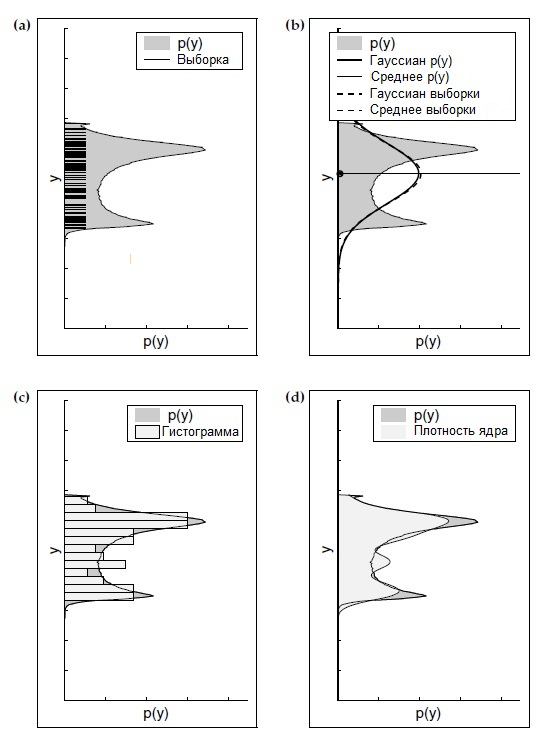
\includegraphics[width=1.1\linewidth]{45orig}}
	\caption{ (  Рис. 4.5 Различные способы извлечения плотностей из частиц. (a) Плотность и аппроксимация набора элементов, (b) гауссова аппроксимация (математическое ожидание и дисперсия), (c) аппроксимация с помощью гистограммы, (d) оценка плотности ядра. Выбор метода аппроксимации сильно зависит от конкретной области применения и вычислительных ресурсов.)}
	\label{fig:45orig}
\end{figure}

\begin{figure}[H]
	\center{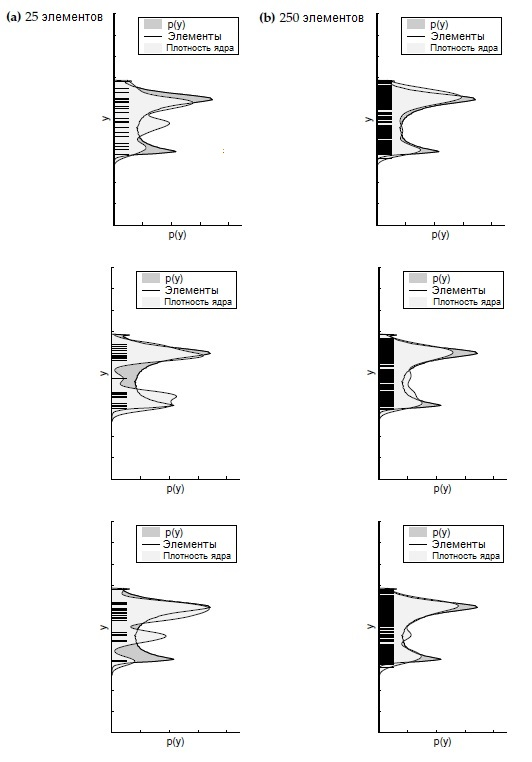
\includegraphics[width=1.1\linewidth]{46orig}}
	\caption{ (  Рис. 4.6 Дисперсия случайной выборки. Элементы извлекаются из гауссовой функции и пропускаются через нелинейную функцию. Показаны элементы и оценки ядер после 25 (левый столбец) и 250 (правый столбец)повторных выборок. В каждой строке показан один эксперимент.)}
	\label{fig:46orig}
\end{figure}

Представим двух одинаковых роботов с идентичными, гауссовыми оценками, выполняющих одинаковые, не подверженные зашумлению, действия. Очевидно, после выполнения действия оба роботы будут иметь одну и ту же оценку состояния. Для имитации этой ситуации будем многократно извлекать значения из гауссовой плотности и пропускать из через нелинейное преобразование. На схемах на Рис. 4.6 показаны результирующие значения и их оценки плотности ядра, а также реальная оценка (серая область). На схемах в верхнем ряду показаны результаты извлечения  из гауссовой функции 25 элементов.
Вопреки ожидаемому результату, некоторые из оценок плотности ядра существенно отличаются от реальной плотности и наблюдается большая дисперсия между разными плотностями ядер. К счастью, дисперсия выборки уменьшается с ростом количества элементов выборки. В нижнем ряду на Рис. 4.6 показаны типичные результаты, полученные для 250 элементов. Очевидно, что увеличение числа элементов ведёт к более точной аппроксимации с меньшей дисперсией. На практике, если выбрано достаточное количество элементов, данных наблюдений, которые выполняет робот, достаточно, чтобы держать оценку на основе выборки «достаточно близко» к настоящей.\\

\textbf{Перевыборка }\\

Дисперсия выборки усиливается при повторной перевыборке.Для понимания проблемы, будет полезно разобрать граничный случай, в котором состояние робота не меняется. Иногда точно известно, что $x_t = x_{t-1}$. Хорошим примером будет задача локализации неподвижного мобильного робота. Давайте ещё более усугубим ситуацию и допустим, что у робота отсутствуют датчики и никакой информации о своём состоянии он получить не может. Очевидно, такой робот никогда ничего не  сможет выяснить об окружении, поскольку оценка в момент времени t будет идентична первоначальной оценке в произвольный  момент времени $t$.

К сожалению, многочастичный фильтр в чистом виде даст другой результат. Изначально, набор частиц будет генерироваться из предыдущего, а частицы – распределены в пространстве состояний. Однако, на шаге перевыборки (строка 8 алгоритма) элемент состояния $x^{[m]}$ в некоторых случаях восстановлен не будет. Поскольку переход состояния детерминирован, новых состояний при проходе по выборке (строка 4) добавлено не будет. С течением времени в силу случайной природы шага перевыборки все больше и больше частиц будет удаляться, при этом новые частицы создаваться не будут. Результат довольно обескураживающий: с вероятностью M будут сохраняться несколько идентичных копий одной и той же частицы. Разнообразие исчезнет в силу повторяющейся перевыборки. Для внешнего наблюдателя может показаться, что робот точно определил состояние окружающей среды – очевидное противоречие в силу того, что у него нет датчиков. 

Этот пример демонстрирует ещё одно ограничение многочастичных фильтров, которое имеет серьёзные практические последствия. Дело в том, что процесс перевыборки вызывает потерю разнообразия в популяции частиц, что ведёт к ошибке аппроксимации. Несмотря на то, что дисперсия самого набора частиц уменьшается, дисперсия набора частиц, как оценивающей функции реального состояния, увеличивается. Управление этой дисперсией, или ошибкой, многочастичного фильтра, очень важно в любой практической реализации. 

УМЕНЬШЕНИЕ ДИСПЕРСИИ \\
Существует две основные стратегии \textit{уменьшения дисперсии}. Во первых, можно уменьшить частоту перевыборки. Если известно, что состояние статическое $(x_t = x_{t-1})$, перевыборка не должна происходить никогда. На примере локализации мобильного робота: когда робот останавливается, перевыборку необходимо приостанавливать (а, вдобавок, неплохо будет приостановить и интеграцию измерений). Даже если состояние меняется, часто полезно уменьшить частоту перевыборки. Несколько измерений всегда можно интегрировать множественным обновлением фактора значимости, как было показано ранее. А именно – держать веса значимости в памяти и обновлять их следующим образом:\\

(4.36)
\begin{equation*}
w_t^{[m]}=\left\{
\begin{array}{ll}
1 & \mbox{ если имеет место перевыборка }\\
p(z_t|x_t^{[m]})\,w_{t-1}^{[m]}& \mbox{ если перевыборка отсутствует }
\end{array}
\right.
\end{equation*}

Решение о необходимости перевыборки достаточно сложное и требует практического опыта:
слишком частая перевыборка увеличивает риск потери разнообразия. Если делать перевыборку слишком редко, множество значений в областях с низкой вероятностью может быть утрачено. Стандартным способом определения того, нужно ли выполнять перевыборку, служит измерение дисперсии весов значимости. Дисперсия весов значимости связана с эффективностью отображения на основе выборки. Если все веса идентичны, то дисперсия равна нулю и перевыборка не нужна. Если, с другой стороны, веса сконцентрированы в небольшом количестве элементов, то дисперсия весов будет велика и необходимо выполнить перевыборку.
 
ВЫБОРКА ПО НИЗКОЙ ДИСПЕРСИИ\\
Вторая стратегия уменьшения ошибки выборки известна как \textit{выборка по низкой дисперсии.} В Таблице 4.4 приводится реализация такого алгоритма выборки. Основной идеей является то, что, при перевыборке вместо независимого выбора элементов (как в случае базового многочастичного фильтра в Таблице 4.3), выбор включает последовательный стохастический процесс.

\begin{table}[H]
\begin{center}
\begin{tabular}{|l|}
\hline
{}\\
1: \hspace{3mm} Algorithm Low\_variance\_sampler $(\mathcal X_t,\mathcal W_t):$ \\
2: \hspace{7mm}$\bar{\mathcal X}_t=0$\\
3:\hspace{7mm}$r=\text{rand}(0;M^{-1})$\\
4:\hspace{7mm}$c=w_t^{[1]}$\\
5:\hspace{7mm}$i=1$\\
6:\hspace{7mm}$\textit{for }\,m=1\,\textit{to}\,M\,\textit{do}$\\
7:\hspace{12mm}$U=r+(m-1)\cdot M^{-1}$\\
8:\hspace{12mm}$\textit{while}\,U>c$\\
9:\hspace{17mm}$i=i+1$\\
10:\hspace{15mm}$c=c+w_t^{[i]}$\\
11:\hspace{11mm}$\textit{endwhile}$\\
12:\hspace{11mm}$\textit{add}\,x_t^{[i]}\,\textit{to}\,\bar{\mathcal X}_t$\\
13:\hspace{6mm}$\textit{endfor}$\\
14:\hspace{6mm}$\textit{return}\,\bar{\mathcal X}_t$\\
{}\\
\hline
\end{tabular}
\caption{(Таблица 4.4 Перевыборка с низкой дисперсией для многочастичного фильтра. Этот алгоритм использует одно случайное число для выборки из набора частиц $\mathcal X$ с ассоциированными весами $\mathcal W$, хотя вероятность частицы быть выбранной все ещё пропорционально ее весу. Алгоритм выборки довольно эффективен и выборка $M$ частиц требует количества операций $O(M)$.)}
\end{center}
\end{table}

Вместо выбора $M$ случайных чисел и отбора частиц, соответствующих этим числам, в этом алгоритме вычисляется единственное случайное число, согласно которому и отбираются элементы, хотя и с вероятностью, пропорциональной весу элемента. Это достигается выбором случайного числа $r$ в интервале $[0; M^{-1} ]$, где $M$ - число элементов для выборки в момент времени $t$. Затем алгоритм в Таблице 4.4 циклически прибавляет фиксированное значение $M_{-1}$ к $r$, отбирая частицу, соответствующую номеру. Любое число $U$ в диапазоне $[0; 1]$ будет указывать только на одну частицу, например, $i$, для которой\\

(4.37)
$$i=\underset{j}{\text{argmin}}\sum_{m=1}^j\,w_t^{[m]}\geq U$$

Цикл с условием в Таблице 4.4 служит двум целям. В нем вычисляется сумма с правой стороны уравнения и дополнительно проверяется, является ли $i$ индексом первой частицы, чтобы соответствующая сумма весов превышала $U$. Отбор выполняется в строке 12. Этот же процесс показан на Рис. 4.7.
\begin{figure}[H]
	\center{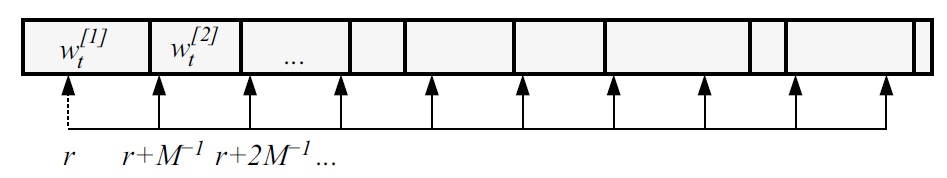
\includegraphics[width=1.1\linewidth]{47orig}}
	\caption{ (  Рис. 4.7 Принцип процедуры перевыборки с низкой дисперсией. Выбирается случайное число $r$, а затем отбираются, только те частицы, которые соответствуют $u=r+(m-1)\cdot M^{-1}$
	где $m = 1, . . . , M$.)}
	\label{fig:47orig}
\end{figure}

У алгоритма отбора с низкой дисперсией три преимущества. Во-первых, он покрывает пространство элементов в значительно более систематической манере, нежели независимый алгоритм отбора. Это очевидно следует из факта, что зависимый алгоритм отбора циклически перебирает все частицы, а не выбирает их случайным образом независимо друг от друга. Во-вторых, если все элементы имеют одинаковые факторы значимости, результирующий набор элементов $\bar{\mathcal X}_t$ эквивалентен $\mathcal X_t$ , поэтому элементы не будут утеряны при перевыборке без интеграции наблюдения в $\mathcal X_t$. В-третьих, алгоритм отбора с низкой дисперсией имеет сложность $O(M)$. Достижение столь же малой сложности для независимой выборки затруднено, поскольку очевидные реализации требуют операций поиска со сложностью $O(\log M)$ для извлечения каждой частицы после выбора случайного числа, что ведёт к сложности всего процесса перевыборки $O(M \log M)$. При использовании многочастичных фильтров очень важно время использования, и, зачастую, эффективная реализация процесса перевыборки означает огромную разницу в практической производительности. Из-за этих причин реализации многочастичных фильтров в робототехнике чаще всего и основаны на обсуждаемых механизмах.

СТРАТИФИЦИРОВАННАЯ ВЫБОРКА\\
В общем же, количество литературы по эффективному отбору выборки огромно. Другим популярным подходом является \textit{стратифицированная выборка}, в которой частицы сгруппированы в подмножества. Отбор элементов из таких наборов выполняется в два этапа. Сначала на основе общего веса частиц в подмножестве определяется количество извлекаемых элементов. На втором этапе отдельные элементы случайным образом извлекаются из каждого множества, используя, например, перевыборку с низкой дисперсией. Такой подход имеет более низкую дисперсию выборки и обычно работает лучше для случаев, когда робот отслеживает несколько отдельных, четко различимых гипотез с помощью одного многочастичного фильтра.\\
 
\textbf{Смещение выборки}\\

Из-за того, что используется только конечное число частиц, возникает систематическое \textit{смещение} в апостериорной оценке. Возьмём, для примера, граничный случай с единственной частицей $M = 1$. В этом случае, цикл в строках с 3 по 7 в Таблице 4.3 будет выполнен только один раз, и $\bar{\mathcal X}_t$ будет содержать единственную частицу, извлечённую из модели движения. Ключевым моментом является то, что перевыборка (строки с 8 по 11 в Таблице 4.3) теперь будет \textit{детерминированным образом} принимать этот элемент, вне зависимости от его фактора значимости $w_t^{[m]}$. Поскольку вероятность измерения $p(z_t | x_t^{[m]})$ не играет никакой роли в результате этого обновления, то же справедливо и для $z_t$. Поэтому, при $M = 1$, многочастичный фильтр генерирует частицы для вероятности $p(x_t | u_{1:t})$ вместо целевой апостериорной $p(x_t | u_{1:t}, z_{1:t})$. Он просто игнорирует все измерения.
Как же это произошло?

Виновником является нормализация, выполняемая на шаге перевыборки. При выборке пропорционально весам значимости (строка 9 алгоритма),
$w_t^{[m]}$ становится собственным нормализатором при $M = 1$:\\

(4.38)
$$p(\text{извлекается}\,x_t^{[m]}\,\text{в строке 9})=\frac{w_t^{[m]}}{w_t^{[m]}}=1$$

В общем случае, проблема состоит в том, что ненормализованные значения $w_t[m]$ извлекаются из $M$-мерного пространства, но, после нормализации, располагаются в пространстве мерности $M - 1$. Так происходит потому, что после нормализации $m$-ый вес можно восстановить из $M - 1$ других весов вычитанием их из
1. К счастью, для больших значений $M$, эффект потери размерности или степеней свободы, становится все менее выраженным.\\

\textbf{Дефицит частиц}\\

Даже при большом числе частиц может сложиться ситуация, когда в окрестностях верного состояния частиц нет. Эта проблема известна как \textit{проблема дефицита частиц}. Она возникает, в основном, когда количество частиц слишком мало, чтобы покрыть все соответствующие области с высокой вероятностью. Однако, можно заметить, что так может случиться с любым многочастичным фильтром, вне зависимости от размера набора частиц $M$.
  
Дефицит частиц происходит в результате дисперсии случайной выборки. Неудачная серия случайных чисел может не содержать ни одной частицы около настоящего состояния. На каждом шаге выборки вероятность, что это случится, больше нуля (хотя обычно экспоненциально меньше, $M$). Таким образом,  при достаточно продолжительном использовании многочастичного фильтра можно получить оценку со сколь угодно большой ошибкой.

На практике проблемы подобного рода возникают только при малом M, относительно пространства всех состояний с высокой вероятностью. Популярным решением проблемы дефицита частиц является добавление небольшого числа случайно сгенерированных частиц в набор после каждой перевыборки, вне зависимости от текущих команд движения и измерения. Такая методология может уменьшить (но не исправить) проблему дефицита, но ценой неверной оценки апостериорной вероятности. Преимущество метода добавления случайных элементов заключается в его простоте: необходима лишь минимальная модификация программного обеспечения. 
В качестве общего правила, добавление случайных элементов следует считать последним средством, которое следует использовать, только если остальные методы исправления проблемы дефицита частиц не работают. 
Альтернативные методы решения проблемы дефицита частиц будут обсуждаться в Главе 8, в контексте локализации робота.

Мы пришли к выводу, что качество отображения на основе выборки возрастает с количеством элементов. Важным вопросом является нахождение количества элементов, которое следует использовать в конкретной задаче оценки. К сожалению, универсального ответа на этот вопрос нет, и, зачастую, требуемое количество элементов может определить только пользователь. Обычно, количество элементов сильно зависит от размерности пространства состояний и степени неопределённости аппроксимируемых фильтром распределений. Так, для однородных распределений требуется намного больше элементов, чем для случаев, сконцентрированных в небольшой области пространства состояний. Более детальное обсуждение размера выборки будет дано в будущих главах в контексте локализации робота и построения карт.\\

\textbf{4.4 Вывод}\\

В этой главе были приведены два непараметрических фильтра Байеса, фильтра на основе гистограмм и многочастичный фильтр. Непараметрические фильтры аппроксимируют апостериорную вероятность с помощью конечного числа значений. При одинаковых допущениях модели системы и формы апостериорного распределения, оба фильтра имеют свойство равномерной сходимости ошибки аппроксимации к нулю при увеличении до бесконечности количества значений, используемых для аппроксимации.\\

• Фильтры на основе гистограмм разбивают пространство состояний на конечное множество выпуклых областей и отображает суммарную апостериорную вероятность каждой области одним числовым значением.\\

• В робототехнике используется множество способов разбиения. В частности, степень разбиения может зависеть (или, наоборот, не зависеть) от структуры окружающей среды. Когда такая зависимость есть, результирующие алгоритмы часто называют «топологическими».\\

• Методы разбиения можно разделить на статические и динамические. Статические разбиения выполняются единообразно, вне зависимости от формы оценки. Динамические разбиения основаны на особенностях оценок робота, когда разбиением пространства состояний пытаются увеличить пространственное разрешение апостериорной вероятности. Динамические разбиения обычно дают лучшие результаты, но более трудно реализуемы.\\
 
• Альтернативным непараметрическим методом является многочастичный фильтр. Многочастичные фильтры представляют апостериорные распределения в виде случайной выборки состояний. Такие элементы называются частицами. Многочастичные фильтры очень легко реализовать, и они являются самыми надёжными из всех алгоритмов байесовских фильтров, представленных в книге. \\

• Существует множество способов уменьшения ошибки многочастотных фильтров. Среди наиболее популярных -  методы уменьшения дисперсии оценки, возникающей в силу случайной природы алгоритма, и регулирования числа частиц в соответствии с сложностью апостериорного распределения. \\ 
  
Алгоритмы фильтров, обсуждаемые в этой и предыдущей главе, образуют основу большинства вероятностных алгоритмов робототехники, которые встретятся в книге.  Представленный здесь материал отражает множество самых популярных сегодня алгоритмов и представлений вероятностной робототехники. \\

\textbf{4.5 Библиографические сведения}\\

Вест и Гаррисон (West and Harrison, 1997) провели детальное исследование нескольких методов, обсуждаемых в этой и предыдущих главах. Гистограммы использовались в статистике многие десятилетия. Стуржес (Sturges, 1926) представил одну из ранних теорем выбора разрешения для аппроксимации с помощью гистограмм, а более современные исследования были проведены Фридманом и Диаконисом (Freedman and Diaconis, 1981). Современный анализ можно найти в работах Скотта (Scott, 1992). После того, как пространство состояний размечается дискретной гистограммой, результирующая задача временного логического вывода становится экземпляром дискретной скрытой марковской модели, ставшей популярной благодаря исследованиям Рабинера и Янга (Rabiner and Juang, 1986). Два современных текста были написаны Макдональдом и Цуккини (MacDonald and Zucchini, 1997) и Элиотом с соавторами (Elliott et al., 1995).

Многочастичные фильтры можно проследить до работ Метрополиса и Улама (Metropolis and Ulam, 1949), которые и изобрели методы Монте-Карло. Более современный вводный текст принадлежит Рубинштейну (Rubinstein, 1981). Метод перевыборки по значимости, входящий в состав многочастичного фильтра, прослеживается до двух основополагающих работ Рубина (Rubin, 1988) и Смита и Гелфанда (Smith and Gelfand, 1992). Стратифицированная выборка была открыта Нейманом (Neyman, 1934). В последние несколько лет многочастичные фильтры интенсивно исследовались в контексте байесовской статистики (Doucet 1998; Kitagawa 1996; Liu and Chen 1998; Pitt and Shephard 1999).
В области искусственного интеллекта, многочастичные фильтры были заново введены под именем "выживание сильнейшего" (Kanazawa et al. 1995). В компьютерном зрении алгоритм, называемый конденсацией, изобретённый Исардом и Блейком (Isard and Blake, 1998) используется в задачах отслеживания объектов. Хороший современный текст по многочастичным фильтрам принадлежит Дюсе с соавторами (Doucet et al., 2001).\\

\textbf{4.6 Упражнения}\\

1. В этом упражнении будет необходимо реализовать фильтр на основе гистограмм для линейной динамической модели, изученный в предыдущей главе.\\

(a) Реализовать фильтр на основе гистограмм для динамической системы, описанной в Упражнении 1 предыдущей главы (см стр. 81????). Использовать фильтр для прогнозирования последовательности апостериорных распределений для $t = 1, 2, . . . , 5$. Для каждого значения $t$, изобразить в виде графика апостериорное распределение $x$ и $\dot{x}$, где $x$ горизонтальная, а $\dot{x}$ - вертикальная ось.\\

(b) Добавить этап обновления измерения  к фильтр на основе гистограмм, как описано в Упражнении 2 предыдущей главы (стр. 82???). Допустим, в момент времени $t = 5$, наблюдается измерение $z = 5$. Определить и изобразить апостериорное распределение перед и после обновления фильтр на основе гистограмм.\\

2. Теперь необходимо реализовать фильтр на основе гистограмм для нелинейного случая, использовав материал Упражнения 4 предыдущей главы (стр. 83???). Напомним, была изучена нелинейная система, определённую тремя переменными состояния, с детерминированным переходом состояний. 


\begin{minipage}{0.3\textwidth}
	\begin{equation*}
	\left(\begin{array}{c}
	x'\\
	y'\\
	\theta'\\
	\end{array}\right)
	\end{equation*}
\end{minipage}
\begin{minipage}{0.3\textwidth}
	\begin{equation*}
	\mbox {=} \hspace{10mm} 
	\left(\begin{array}{c}
	x+\cos\theta\\
	y+\sin\theta\\
	\theta\\
	\end{array}\right)
	\end{equation*}
\end{minipage}\\

Начальная оценка состояния задана следующим образом:\\

\begin{minipage}{0.3\textwidth}
	\begin{equation*}
	\mu=
	\left(\begin{array}{ccc}
	0 & 0 & 0\\
	\end{array}\right)
	\end{equation*}
\end{minipage}
\begin{minipage}{0.3\textwidth}
	\begin{equation*}
	\mbox {и} \hspace{10mm} \varSigma=
	\left(\begin{array}{ccc}
	0,01 & 0 & 0\\
	0 & 0,01 & 0\\
	0 & 0 & 10000\\
	\end{array}\right)
	\end{equation*}
\end{minipage}\\

(a) Предложить подходящую начальную оценку для фильтра на основе гистограмм, отражающую информацию об априорном гауссовом распределении.\\

(b) Реализовать фильтр на основе гистограмм и выполнить этап прогнозирования. Сравнить результирующее апостериорное распределение с аналогичным, полученным с помощью EKF и интуитивного анализа. Что можно сказать о разрешении по координатам $x$, $y$ и ориентации $\theta$ с помощью фильтра на основе гистограмм?\\

(c) Интегрировать в оценку данные измерения. Как и прежде, измерение представляет собой зашумлённую проекцию $x$-координаты робота с ковариацией $Q = 0,01$. Реализовать этот шаг, вычислить, изобразить на графике, и сравнить с результатами EKF и интуитивного анализа.\\
 
Примечание: При изображении результатов фильтра на основе гистограмм на графике,  показать несколько графиков вероятности, по одному для каждого дискретного диапазона в пространстве всех значений $\theta$.\\

3. В тексте уже обсуждался эффект использования единственной частицы. Каков будет результат использования $M = 2$ частиц при фильтрации? Можно ли дать пример смещённого апостериорного распределения? Если да, то каково смещение?\\

4. Выполнить Упражнение 1, используя вместо гистограмм многочастичные фильтры, изобразить на графике и объяснить результат.\\

5. Выполнить Упражнение 2, используя вместо гистограмм многочастичные фильтры, изобразить на графике и объяснить результат. Исследовать эффект влияния различного количества частиц на результат.\\





\end{document}